\chapter*{Appendices}
\label{appendices}
%###################################################################################
%###################### Appendix A          ########################################
%###################################################################################
%\newpage
\addcontentsline{toc}{section}{Appendix A: Abbreviations}
\section*{Appendix A: Abbreviations}
\begin{center}
\begin{tabular}{ll}
\textbf{FoV}	&	Field of View\\
\textbf{LiDAR}	&	Light Detection and Ranging\\
\textbf{ODM}	&	Occlusion Degree Model (mathematical model)\\
\textbf{RGBA}	&	Red, Green, Blue and Alpha (opacity index)\\
\textbf{ROI}	&	Region of Interest\\
\textbf{CPO}	&	Camera Placement Optimisation\\
%\textbf{abk}	&	erklärung\\
%\textbf{abk}	&	erklärung\\
%\textbf{abk}	&	erklärung\\
%\textbf{abk}	&	erklärung\\
%\textbf{abk}	&	erklärung\\
%\textbf{abk}	&	erklärung\\
%\textbf{abk}	&	erklärung\\
%\textbf{abk}	&	erklärung\\
\end{tabular}
\end{center}

%###################################################################################
%###################### Appendix B          ########################################
%###################################################################################
\newpage
\addcontentsline{toc}{section}{Appendix B: Link to GitLab repository}
\section*{Appendix B: GitLab Link}

Here is the link to my GitLab repository, where the Python scripts used for implementation of our approach are available in folder \textit{camera\_optimization}: \url{https://git.tu-berlin.de/georgik1609/bachelor_thesis}, visited on 21/12/2022.

\newpage
\addcontentsline{toc}{section}{Appendix C: Images of town and vehicles}
\section*{Appendix C: Images of town and vehicles}
In this section we present pictures of the town and vehicles with their bounding boxes to get a visual idea of the environment and its actors that participated in our simulations. The lightbulbs and projectors are shown because images were made in editor mode, but have nothing to do with the thesis.
\begin{figure} [h!]
    \centering
    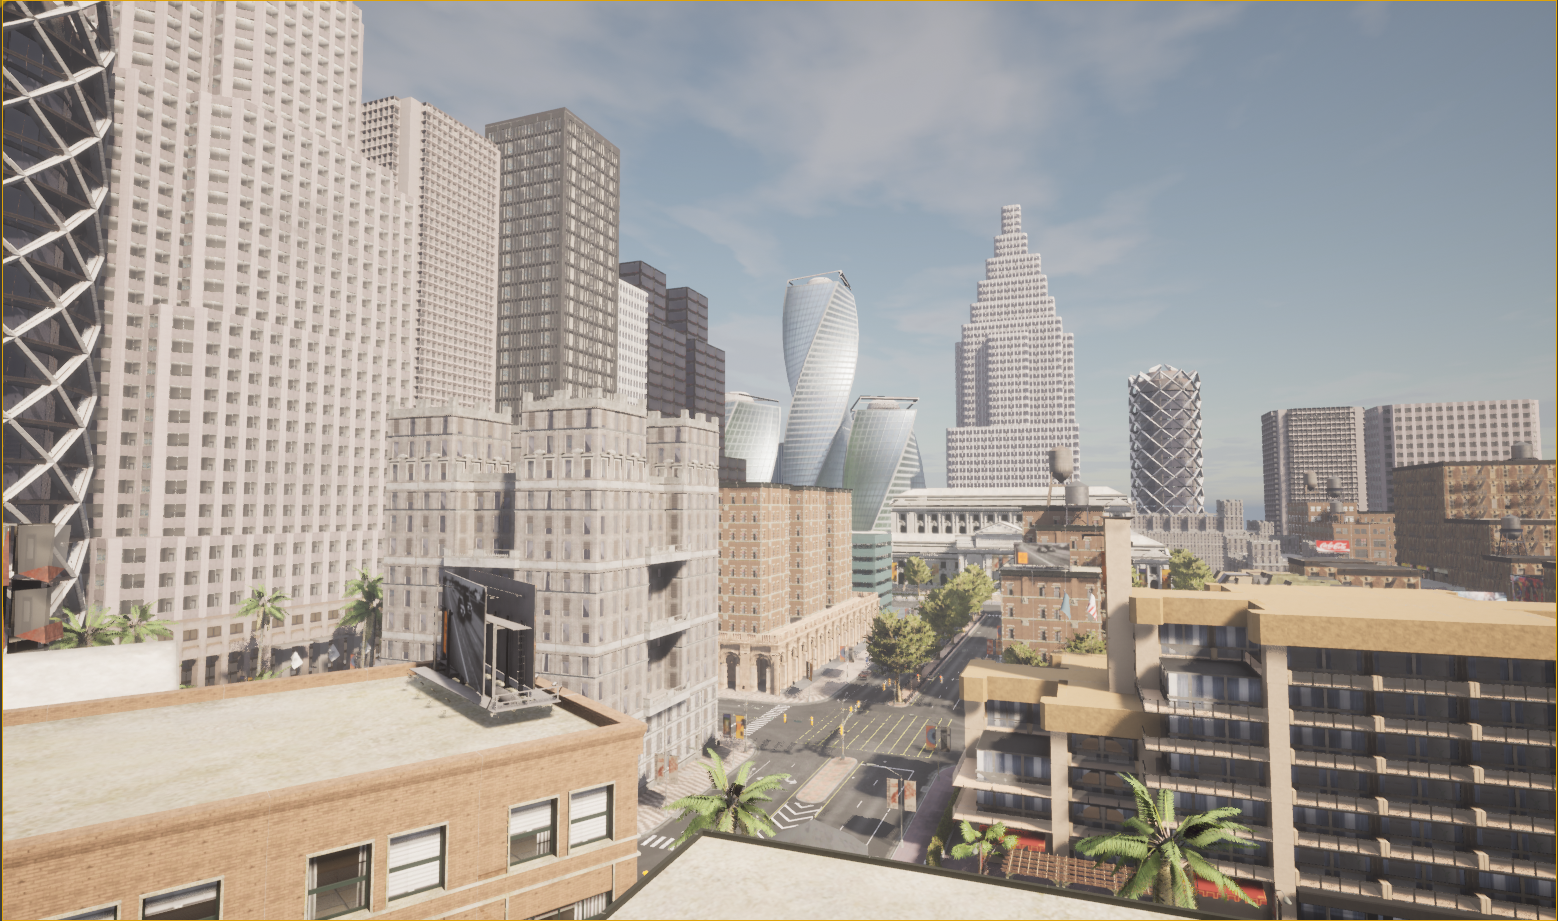
\includegraphics[width=\textwidth]{images/experiment_city.png}
    \caption[Environment for experiments]{This picture shows how the city which we used for our simulations is designed. In the middle, the junction can be seen.}
    \label{fig:city_experiments}
\end{figure}

\newpage
\begin{figure} [h!]
    \centering
    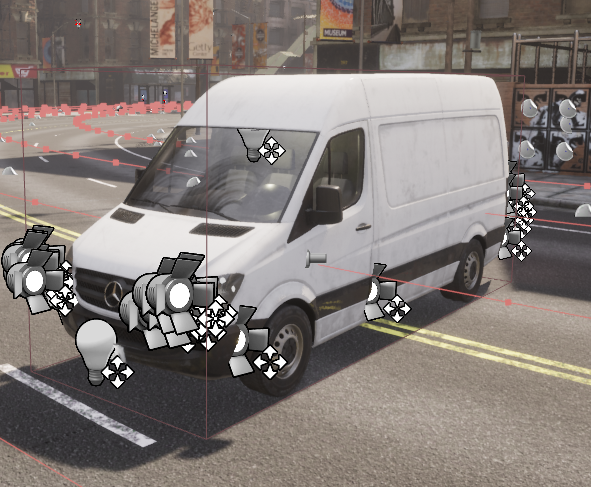
\includegraphics[width=0.5\textwidth]{images/mercedes_sprinter.png}
    \caption[Mercedes Sprinter]{Mercedes Sprinter}
    \label{fig:mercedes_sprinter}
\end{figure}

\begin{figure} [h!]
    \centering
    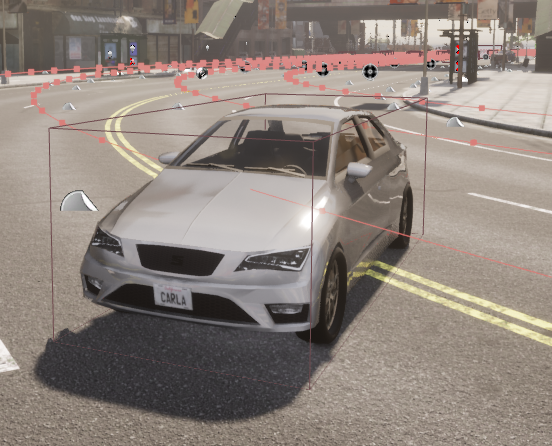
\includegraphics[width=0.5\textwidth]{images/seat_leon.png}
    \caption[Seat Leon]{Seat Leon}
    \label{fig:seat_leon}
\end{figure}

\begin{figure} [h!]
    \centering
    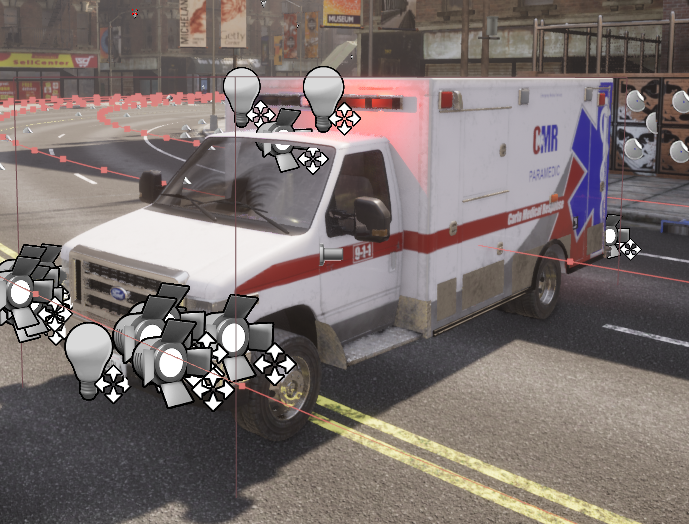
\includegraphics[width=0.5\textwidth]{images/ambulance.png}
    \caption[Ambulance]{Ambulance}
    \label{fig:ambulance}
\end{figure}

\begin{figure} [h!]
    \centering
    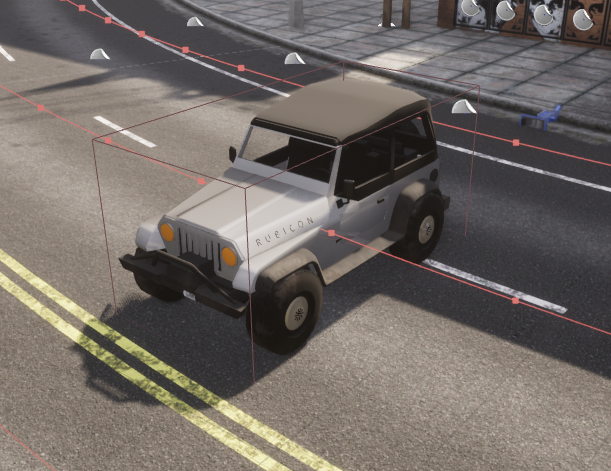
\includegraphics[width=0.5\textwidth]{images/jeep_wrangler_rubicon.png}
    \caption[Jeep Wrangler Rubicon]{Jeep Wrangler Rubicon}
    \label{fig:jeep_wrangler}
\end{figure}

\begin{figure} [h!]
    \centering
    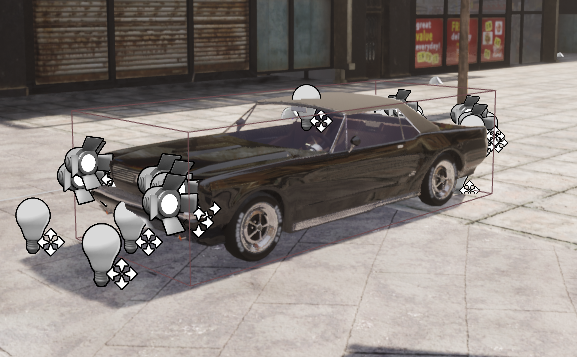
\includegraphics[width=0.5\textwidth]{images/ford_mustang.png}
    \caption[Ford Mustang]{Ford Mustang}
    \label{fig:ford_mustang}
\end{figure}

\newpage
\addcontentsline{toc}{section}{Appendix D: Heatmaps from experiments}
\section*{Appendix D: Heatmaps from experiments} \label{appendix_heatmaps}

Here we display the rest of our heatmaps, which can be used to get a clear idea of the camera's performance in each executed simulation. To clarify, from Figure \ref{fig:pos2_8m} on, all the heatmaps represent the results from the second experiment for a camera placed at 8-meter height.

\begin{figure}[!htb]
\minipage{0.5\textwidth}
  \includesvg[width=\linewidth]{images/position0/pos0_6m.svg}
  \caption{Pos.1 at 6 m height}\label{fig:pos1_6m}
\endminipage\hfill
\minipage{0.5\textwidth}
  \includesvg[width=\linewidth]{images/position0/pos0_7m.svg}
  \caption{Pos.1 at 7 m height}\label{fig:pos1_7m}
\endminipage\hfill
\end{figure}

\begin{figure}[!htb]
\minipage{0.5\textwidth}
  \includesvg[width=\linewidth]{images/position0/pos0_9m.svg}
  \caption{Pos.1 at 9 m height}\label{fig:pos1_9m}
\endminipage\hfill
\minipage{0.5\textwidth}
  \includesvg[width=\linewidth]{images/position1/pos1_6m.svg}
  \caption{Pos.2 at 6 m height}\label{fig:pos2_6m}
\endminipage\hfill
\end{figure}

\begin{figure}[!htb]
\minipage{0.5\textwidth}
  \includesvg[width=\linewidth]{images/position1/pos1_7m.svg}
  \caption{Pos.2 at 7 m height}\label{fig:pos2_7m}
\endminipage\hfill
\minipage{0.5\textwidth}
  \includesvg[width=\linewidth]{images/position1/pos1_9m.svg}
  \caption{Pos.2 at 9 m height}\label{fig:pos2_9m}
\endminipage\hfill
\end{figure}

\begin{figure}[!htb]
\minipage{0.5\textwidth}
  \includesvg[width=\linewidth]{images/position2/pos2_6m.svg}
  \caption{Pos.3 at 6 m height}\label{fig:pos3_6m}
\endminipage\hfill
\minipage{0.5\textwidth}
  \includesvg[width=\linewidth]{images/position2/pos2_7m.svg}
  \caption{Pos.3 at 7 m height}\label{fig:pos3_7m}
\endminipage\hfill
\end{figure}

\begin{figure}[!htb]
\minipage{0.5\textwidth}
  \includesvg[width=\linewidth]{images/position2/pos2_9m.svg}
  \caption{Pos.3 at 9 m height}\label{fig:pos3_9m}
\endminipage\hfill
\minipage{0.5\textwidth}
  \includesvg[width=\linewidth]{images/position3/pos3_6m.svg}
  \caption{Pos.4 at 6 m height}\label{fig:pos4_6m}
\endminipage\hfill
\end{figure}

\begin{figure}[!htb]
\minipage{0.5\textwidth}
  \includesvg[width=\linewidth]{images/position3/pos3_7m.svg}
  \caption{Pos.4 at 7 m height}\label{fig:pos4_7m}
\endminipage\hfill
\minipage{0.5\textwidth}
  \includesvg[width=\linewidth]{images/position3/pos3_9m.svg}
  \caption{Pos.4 at 9 m height}\label{fig:pos4_9m}
\endminipage\hfill
\end{figure}

\begin{figure}[!htb]
\minipage{0.5\textwidth}
  \includesvg[width=\linewidth]{images/position4/pos4_6m.svg}
  \caption{Pos.5 at 6 m height}\label{fig:pos5_6m}
\endminipage\hfill
\minipage{0.5\textwidth}
  \includesvg[width=\linewidth]{images/position4/pos4_7m.svg}
  \caption{Pos.5 at 7 m height}\label{fig:pos5_7m}
\endminipage\hfill
\end{figure}

\begin{figure}[!htb]
\minipage{0.5\textwidth}
  \includesvg[width=\linewidth]{images/position4/pos4_9m.svg}
  \caption{Pos.5 at 9 m height}\label{fig:pos5_9m}
\endminipage\hfill
\minipage{0.5\textwidth}
  \includesvg[width=\linewidth]{images/position5/pos5_6m.svg}
  \caption{Pos.6 at 6 m height}\label{fig:pos6_6m}
\endminipage\hfill
\end{figure}

\begin{figure}[!htb]
\minipage{0.5\textwidth}
  \includesvg[width=\linewidth]{images/position5/pos5_7m.svg}
  \caption{Pos.6 at 7 m height}\label{fig:pos6_7m}
\endminipage\hfill
\minipage{0.5\textwidth}
  \includesvg[width=\linewidth]{images/position5/pos5_9m.svg}
  \caption{Pos.6 at 9 m height}\label{fig:pos6_9m}
\endminipage\hfill
\end{figure}

\begin{figure}[!htb]
\minipage{0.5\textwidth}
  \includesvg[width=\linewidth]{images/position6/pos6_6m.svg}
  \caption{Pos.7 at 6 m height}\label{fig:pos7_6m}
\endminipage\hfill
\minipage{0.5\textwidth}
  \includesvg[width=\linewidth]{images/position6/pos6_7m.svg}
  \caption{Pos.7 at 7 m height}\label{fig:pos7_7m}
\endminipage\hfill
\end{figure}

\begin{figure}[!htb]
\minipage{0.5\textwidth}
  \includesvg[width=\linewidth]{images/position6/pos6_9m.svg}
  \caption{Pos.7 at 9 m height}\label{fig:pos7_9m}
\endminipage\hfill
\minipage{0.5\textwidth}
  \includesvg[width=\linewidth]{images/position7/pos7_6m.svg}
  \caption{Pos.8 at 6 m height}\label{fig:pos8_6m}
\endminipage\hfill
\end{figure}

\begin{figure}[!htb]
\minipage{0.5\textwidth}
  \includesvg[width=\linewidth]{images/position7/pos7_7m.svg}
  \caption{Pos.8 at 7 m height}\label{fig:pos8_7m}
\endminipage\hfill
\minipage{0.5\textwidth}
  \includesvg[width=\linewidth]{images/position7/pos7_9m.svg}
  \caption{Pos.8 at 9 m height}\label{fig:pos8_9m}
\endminipage\hfill
\end{figure}

\begin{figure}[!htb]
\minipage{0.5\textwidth}
  \includesvg[width=\linewidth]{images/position1/pos1_8m.svg}
  \caption{Pos.2 Seat and Jeep}\label{fig:pos2_8m}
\endminipage\hfill
\minipage{0.5\textwidth}
  \includesvg[width=\linewidth]{images/mustang_sprinter/sprinter_mustang_pos1.svg}
  \caption{Pos.2 Ford and Mercedes}\label{fig:pos2_ford_merc}
\endminipage\hfill
\end{figure}

\newpage
\begin{figure}[!htb]
\minipage{0.5\textwidth}
  \includesvg[width=\linewidth]{images/sprinter_ambulance/ambulance_sprinter_pos1.svg}
  \caption{Pos.2 Ambulance and Mercedes}\label{fig:pos2_amb_merc}
\endminipage\hfill
\minipage{0.5\textwidth}
  \includesvg[width=\linewidth]{images/position4/pos4_8m.svg}
  \caption{Pos.5 Seat and Jeep}\label{fig:pos5_8m}
\endminipage\hfill
\end{figure}

\begin{figure}[!htb]
\minipage{0.5\textwidth}
  \includesvg[width=\linewidth]{images/mustang_sprinter/sprinter_mustang_pos4.svg}
  \caption{Pos.5 Ford and Mercedes}\label{fig:pos5_ford_merc}
\endminipage\hfill
\minipage{0.5\textwidth}
  \includesvg[width=\linewidth]{images/sprinter_ambulance/ambulance_sprinter_pos4.svg}
  \caption{Pos.5 Ambulance and Mercedes}\label{fig:pos5_amb_merc}
\endminipage\hfill
\end{figure}

\begin{figure}[!htb]
\minipage{0.5\textwidth}
  \includesvg[width=\linewidth]{images/position6/pos6_8m.svg}
  \caption{Pos.7 Seat and Jeep}\label{fig:pos7_8m}
\endminipage\hfill
\minipage{0.5\textwidth}
  \includesvg[width=\linewidth]{images/mustang_sprinter/sprinter_mustang_pos6.svg}
  \caption{Pos.7 Ford and Mercedes}\label{fig:pos7_ford_merc}
\endminipage\hfill
\end{figure}

\newpage
\begin{figure}[!htb]
\minipage{0.5\textwidth}
    \includesvg[width=\linewidth]{images/sprinter_ambulance/ambulance_sprinter_pos6.svg}
  \caption{Pos.7 Ambulance and Mercedes}\label{fig:pos7_amb_merc}
\endminipage\hfill
\end{figure}

% \newpage
% %change this
% \addcontentsline{toc}{section}{Appendix C: {\LaTeX} Help}
% \section*{Appendix C: {\LaTeX} Help}
% %remove this
% %###################################################################################
%###################### HowTo               ########################################
%###################################################################################
\subsection*{How to Use This Template}
\begin{itemize}
\item Remove all of my text which is mostly labeled with DELETEME
\item Change the information in the 00a\_title\_page.tex file
\item Use the information written in this section
\item Ask you supervizor to help you
\item If I am not your supervizor and noone else can help you, write me an email (aubrey.schmidt@dai-labor.de)
\end{itemize}

%###################################################################################
%###################### Citations           ########################################
%###################################################################################
\subsection*{Citations}
Citing is one of the essential points you need to do in you thesis. Statements not basing on results of your own research\footnote{in what ever context} not being cited represent a breach on the rules of scientific working. Therefore, you every statement needs to be cited basing on information that other people can cross-check. A common way of citing in technical papers is: 
\begin{itemize}
\item Oberheide et al.~\cite{oberheide:2008:cloudav} state that the average time for an anti-virus enginge to be updated with a signature to detect an unknown threat is 48 days.
\end{itemize}
Note: et al. is used when the paper was written by more than two people. Check the code of this section to learn how to cite from a technical perspective.

Note: you can change the citation style in the \texttt{thesis.tex} file, e.g. to harvard style citations. Instructions on this can also be found in this file.

You should not cite anything that can be changed, e.g. it is not that good citing web pages since they might get updated changing the cited content. There are no clear quality measures on citing sources but aubrey believes that the following list is true for several cases, starting with highest quality:
\begin{enumerate}
\item Journal article or book
\item Conference paper
\item Workshop paper
\item Technical report
\item Master thesis
\item Bachelor thesis
\item General Web reference
\end{enumerate}
There might be workshop papers that have a higher quality than some journal papers. Therefore this list only gives you a hint on possible quality measures. Another measure can be whether a paper was indexed by ACM/IEEE, although this is not a strong indicator.

%###################################################################################
%###################### Papers             ########################################
%###################################################################################
\subsection*{Finding and Handling Citation Sources}
Following ressources are required for finding and handling articles, books, papers and sources.
\begin{itemize}
\item your primary resource will be \url{http://scholar.google.com}
\item \url{http://www.google.com} might also be used
\item \url{wikipedia.com} can be a good start for finding relevant papers on your topic
\item you should download and install JabRef or a similar tool \url{http://jabref.sourceforge.net/}
\item you should point JabRef to the mybib.bib file
\item you should immediately enter a relevant paper to JabRef, additionally, you should write a short summary on it; else, you will do this work at least twice.
\end{itemize}

%###################################################################################
%###################### General             ########################################
%###################################################################################
\subsection*{General Advices}
\begin{itemize}
\item Do not take care of design, \LaTeX will do this for you. If you still feel that you need to take care of this, do this when you have finished writing, else you will end up in a lot of double and triple work.
\item \LaTeX will do exactly that you will tell it to do. If you have problems with this, go for google or ask you supervizor
\item use labels in order to be able to reference to chapters, section, subsections, figures, tables, etc. ...
\end{itemize}

%###################################################################################
%###################### Commands            ########################################
%###################################################################################
\subsection*{General Commands}
\begin{itemize}
\item check \url{http://en.wikibooks.org/wiki/LaTeX}
\item check \url{http://www.uni-giessen.de/hrz/tex/cookbook/cookbook.html} German
\end{itemize}
Please also check the following source~\cite{latexcookbook2007}.

%###################################################################################
%###################### Code                ########################################
%###################################################################################
\newpage
\subsection*{Code}
This section shows you how to get your code into a \LaTeX document. See code for options.
\lstinputlisting[language=JAVA,xleftmargin=8mm,]{help/Example.java}


\lstset{ %
language=Java,   	             % the language of the code
numbers=left,
basicstyle=\scriptsize,       % the size of the fonts that are used for the code
numbers=left,                   % where to put the line-numbers
numberstyle=\scriptsize,      % the size of the fonts that are used for the line-numbers
stepnumber=1,                   % the step between two line-numbers. If it's 1, each line 
                                % will be numbered
numbersep=5pt,                  % how far the line-numbers are from the code
backgroundcolor=\color{white},  % choose the background color. You must add \usepackage{color}
showspaces=false,               % show spaces adding particular underscores
showstringspaces=false,         % underline spaces within strings
showtabs=false,                 % show tabs within strings adding particular underscores
frame=single,                   % adds a frame around the code
tabsize=2,                      % sets default tabsize to 2 spaces
captionpos=b,                   % sets the caption-position to bottom
breaklines=true,                % sets automatic line breaking
breakatwhitespace=false,        % sets if automatic breaks should only happen at whitespace
title=\lstname,                 % show the filename of files included with \lstinputlisting;
                                % also try caption instead of title
xleftmargin=8mm,
framexleftmargin=4mm,           
escapeinside={\%*}{*)},         % if you want to add a comment within your code
morekeywords={*,...}            % if you want to add more keywords to the set
}
\begin{lstlisting}[float=h, caption=Example code is presented here, label=list:code, frame=single]
class Beispiel{

	public static void main(String args[]){
	
		System.out.println("Hello World");
		
	}
	
}
\end{lstlisting}

%###################################################################################
%###################### Figures             ########################################
%###################################################################################
\newpage
\subsection*{Figures}
This section describes how to include images to your document. Information was taken from \url{http://en.wikibooks.org/wiki/LaTeX/Floats,_Figures_and_Captions}, visited on 05/08/2011. Please make sure to use original vector graphics as basis since image quality might be used as weak indicator for thesis quality. For this, try to find find files in \texttt{.SVG} or \texttt{.PDF} format. Exporting a \texttt{.PNG} or \texttt{.JPG} to \texttt{.PDF} will not work since data was already lost while exporting it to these formats. This is the case for most Web graphics. Wikipedia startet entering most in images in \texttt{.SVG} which easily can be transformed to \texttt{.PDF}, but please do not forget proper citations.

%use a modifier to decide where you desire Latex should put the image: (h)ere, (t)op, (b)ottom, or nothing more than that image on a (p)age
\begin{figure}[h]%[htbp]
%this will center your image
\centering
%this will include your image
\includegraphics[width=0.15\textwidth]{template/TUBerlin_Logo_rot_hell}
%this is the caption + label. the label will not be printed in the caption. Moving the label out of the caption can result in problems.
\caption[Including an Image]{Including an image; in this case a PDF. Please note that the caption is placed below the image.\label{fig:help1}}
\end{figure}

\begin{figure}[h]
%this will center your image
\centering
%this will include your image

\includegraphics[width=0.25\textwidth]{template/aot_logo}
%this is the caption + label. the label will not be printed in the caption. Moving the label out of the caption can result in problems.
\caption[Short caption for list of figures]{See code for caption options: this is a long caption which is printed in the Text. Additionally, image size was increased\label{fig:help2}}
\end{figure}


\begin{figure}[h]
  \centering
  \subfloat[Small]{\label{fig:tub1}\includegraphics[width=0.1\textwidth]{template/TUBerlin_Logo_rot_hell}}                
  \subfloat[Large]{\label{fig:tub2}\includegraphics[width=0.3\textwidth]{template/TUBerlin_Logo_rot_hell}}
  \subfloat[Medium]{\label{fig:tub3}\hspace{2cm}\includegraphics[width=0.2\textwidth]{template/TUBerlin_Logo_rot_hell}}
  \caption[Placing images side by side]{Placing images side by side using the subfig package. Space between the images can be adjusted.\label{fig:tuball}}
\end{figure}


%###################################################################################
%###################### Tables              ########################################
%###################################################################################
\newpage
\subsection*{Tables}
Here, you will find some example tables.The tables were taken from \url{http://en.wikibooks.org/wiki/LaTeX/Tables}, visited on 05/08/2011. Table environment was added plus caption and label. For code, check \url{__help/latex_hinweise.tex}.

\begin{table}[h]
\caption{Simple table using vertical lines. Note that the caption is always above the table! Please check code for finding the right place for the table label.\label{tab:help1}}
\centering
  \begin{tabular}{ l | c || r | }
    \hline
    1 & 2 & 3 \\ \hline
    4 & 5 & 6 \\ \hline
    7 & 8 & 9 \\
    \hline
  \end{tabular}
\end{table}

\begin{table}[h]
\caption{Table using vertical and horizontal lines\label{tab:help2}}
\centering
\begin{tabular}{|r|l|}
  \hline
  7C0 & hexadecimal \\
  3700 & octal \\ \cline{2-2}
  11111000000 & binary \\
  \hline \hline
  1984 & decimal \\
  \hline
\end{tabular}
\end{table}

\begin{table}[h]
\caption{Table with column width specification on last column\label{tab:help3}}
\centering
    \begin{tabular}{ | l | l | l | p{5cm} |}
    \hline
    Day & Min Temp & Max Temp & Summary \\ \hline
    Monday & 11C & 22C & A clear day with lots of sunshine.  
    However, the strong breeze will bring down the temperatures. \\ \hline
    Tuesday & 9C & 19C & Cloudy with rain, across many northern regions. Clear spells
    across most of Scotland and Northern Ireland,
    but rain reaching the far northwest. \\
    \hline
    \end{tabular}
\end{table}

\begin{table}[h]
\caption{Table using multi-column and multirow\label{tab:help4}}
\centering
\begin{tabular}{|l|l|l|}
\hline
\multicolumn{3}{|c|}{Team sheet} \\
\hline
Goalkeeper & GK & Paul Robinson \\ \hline
\multirow{4}{*}{Defenders} & LB & Lucus Radebe \\
 & DC & Michael Duberry \\
 & DC & Dominic Matteo \\
 & RB & Didier Domi \\ \hline
\multirow{3}{*}{Midfielders} & MC & David Batty \\
 & MC & Eirik Bakke \\
 & MC & Jody Morris \\ \hline
Forward & FW & Jamie McMaster \\ \hline
\multirow{2}{*}{Strikers} & ST & Alan Smith \\
 & ST & Mark Viduka \\
\hline
\end{tabular}
\end{table}






